\documentclass{beamer}

\usepackage[utf8]{inputenc}
\usepackage[T1]{fontenc}
\usepackage{lmodern}
\usepackage[scale=2]{ccicons}
\usepackage{tikz}

\usepackage[english]{babel}
% \usepackage[english, polish]{babel}

\usepackage{listings}
\lstset{basicstyle=\ttfamily\footnotesize,breaklines=true}

\usepackage{siunitx}
\usepackage{pifont}
\usepackage{amsmath,amssymb,amsfonts}
\usepackage{graphicx}
\usepackage[export]{adjustbox}
\usepackage{float}
\usepackage{xcolor}
\usepackage{xspace}
\usepackage{setspace}

\usetheme{CambridgeUS}
\useoutertheme{miniframes}
\usecolortheme{dolphin}
\usefonttheme{professionalfonts}
\beamertemplatenavigationsymbolsempty

\setbeamertemplate{background}{
    \tikz[overlay,remember picture]\node[opacity=0.09]at (current page.center){
        
\includegraphics[width=7cm]{images/WF_sygnet_czarny.png}
    };
}

\defbeamertemplate{headline}{pwtemplate}{
    \leavevmode
    \hbox{
        \begin{beamercolorbox}[wd=\paperwidth,ht=2.25ex,dp=1ex,right]{title in head/foot}
            \usebeamerfont{title in head/foot}
            \insertframenumber/\inserttotalframenumber\hspace*{2em}
        \end{beamercolorbox}}
    \vskip0pt
}

\defbeamertemplate{footline}{pwtemplate}{ % gray!0 is white
    \leavevmode
    \setbeamercolor{lfooterbox}{bg=gray!0}
    \begin{beamercolorbox}[wd=.33\paperwidth,ht=7pt,dp=4pt,center]{lfooterbox}
        % \usebeamerfont{author in head/foot}
        
\includegraphics[scale=0.07]{images/WF_PW_sygnet_EN_czarny_RGB.png}
    \end{beamercolorbox}%
    \setbeamercolor{cfooterbox}{bg=gray!0}
    \begin{beamercolorbox}[wd=.34\paperwidth,ht=7pt,dp=4pt,center]{cfooterbox}
        % \usebeamerfont{date in head/foot}
    \end{beamercolorbox}%
    \setbeamercolor{rfooterbox}{bg=gray!0}
    \begin{beamercolorbox}[wd=.33\paperwidth,ht=7pt,dp=4pt,right]{rfooterbox}
        \usebeamerfont{title in head/foot}
        \insertshortauthor \hspace*{2em}
    \end{beamercolorbox}
}



\newcommand{\todo}[1]{\textcolor{red}{TODO: #1}}
\newcommand{\keV}[0]{\si{\kilo\electronvolt}}
\newcommand{\MeV}[0]{\si{\mega\electronvolt}}
\newcommand{\GeV}[0]{\si{\giga\electronvolt}}

\newcommand{\aegis}{AE$\overline{\textrm{g}}$IS\xspace}

\newcommand{\imagesource}[1]{
    \begin{spacing}{0.5}
        \texttt{\textit{ \tiny{source: #1}}}
    \end{spacing}
}

\newenvironment{columnframe}[1]{
    \begin{frame}[environment=columnframe,fragile]{#1}
        \begin{columns}
            }{
        \end{columns}
    \end{frame}
}




\title{Photonis PET Machine BGO PMT's}
    \subtitle{\textit{An introduction}}
\author[T. Fic]{Tobiasz Fic}
\institute[WUT]{Faculty of Physics, Warsaw University of Technology}

\date{2 December 2024}

\begin{document}

\begin{frame}
    \maketitle
\end{frame}

\section{What are we measuring?}

\begin{columnframe}{Contact}
    \begin{column}{0.5\textwidth}
        \begin{figure}
            \centering
            
\includegraphics[width=0.6\textwidth]{images/logo-PW.png}
        \end{figure}
    \end{column}
    \begin{column}{0.5\textwidth}
        My name is Tobiasz, I am a masters student at the Faculty of Physics at Warsaw University of Technology, working with the \aegis collaboration. \vspace{0.5cm}

        \small{email: \href{mailto:tobiasz.fic.stud@pw.edu.pl}{tobiasz.fic.stud@pw.edu.pl}

            or

            \href{mailto:tobiasz.fic@cern.ch}{tobiasz.fic@cern.ch}}
        \vspace{0.5cm}

        My supervisor is Georgy Kornakov (\href{mailto:georgy.kornakov@cern.ch}{georgy.kornakov@cern.ch})
    \end{column}
\end{columnframe}

\begin{columnframe}{Overall goal}
    \begin{column}{0.5\textwidth}
        \begin{figure}
            \centering
            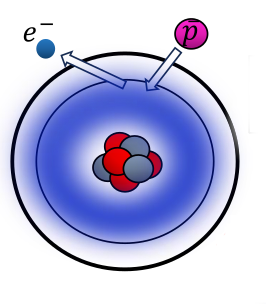
\includegraphics[width=0.6\textwidth]{images/antiprotonic_atom.png}
        \end{figure}
    \end{column}
    \begin{column}{0.5\textwidth}
        \begin{itemize}
            \item Recently we have been trying to build a calorimeter for measuring the transition radiation of antiprotonic atoms.
            \item An antiprotonic atom is an atom with an electron replaced by an antiproton.
        \end{itemize}
    \end{column}
\end{columnframe}

\begin{frame}{Life cycle of an antiprotonic atom}
    \begin{figure}
        \centering
        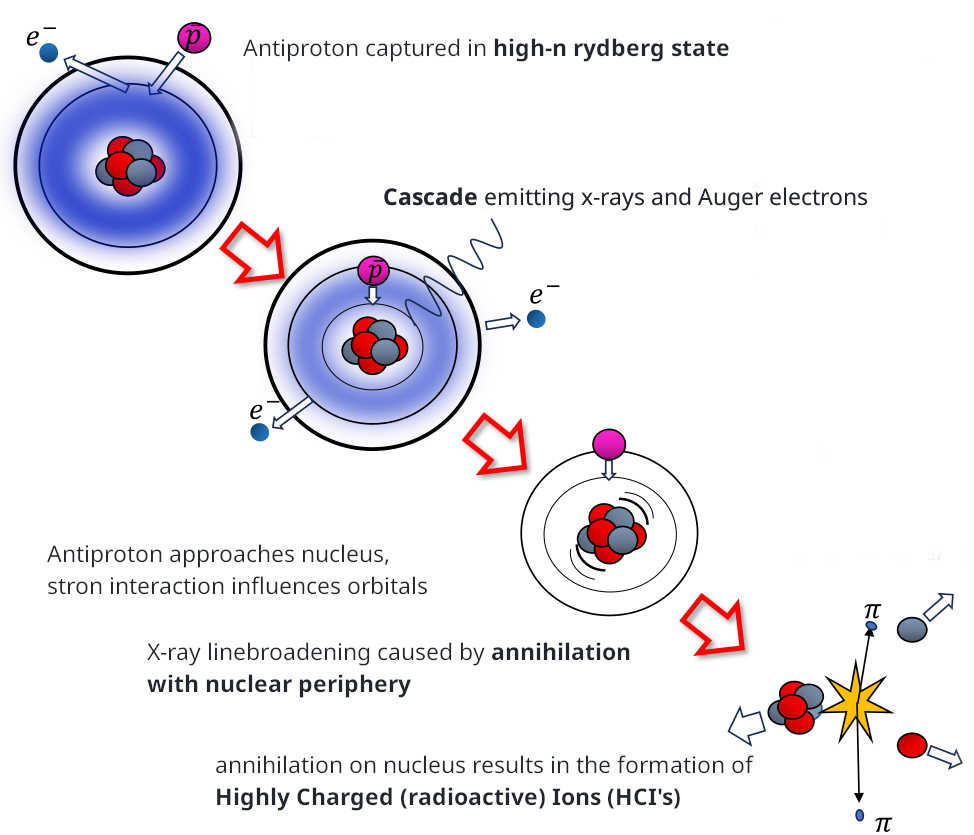
\includegraphics[width=0.75\textwidth]{images/formation_of_hci.png}
    \end{figure}
\end{frame}

\begin{columnframe}{Energy detection range}
    \begin{column}{0.5\textwidth}
        \begin{figure}
            \centering
            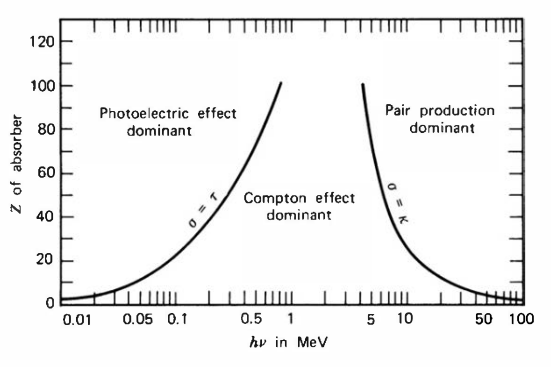
\includegraphics[width=0.9\textwidth]{images/effect_dominance_knoll.png}
        \end{figure}
    \end{column}
    \begin{column}{0.5\textwidth}
        \begin{itemize}
            \item The photons we would like to measure are in the X-ray to soft gamma range (1 \keV to 10 \MeV)
            \item We are aware that this might not be possible since the tubes are made to register 511 \keV electron-positron annihilations.
            \item The sources we have only go up to around 1.3 \MeV
        \end{itemize}
    \end{column}
\end{columnframe}

\section{Detector specs}

\begin{frame}{Dimensions}
    \begin{figure}
        \centering
        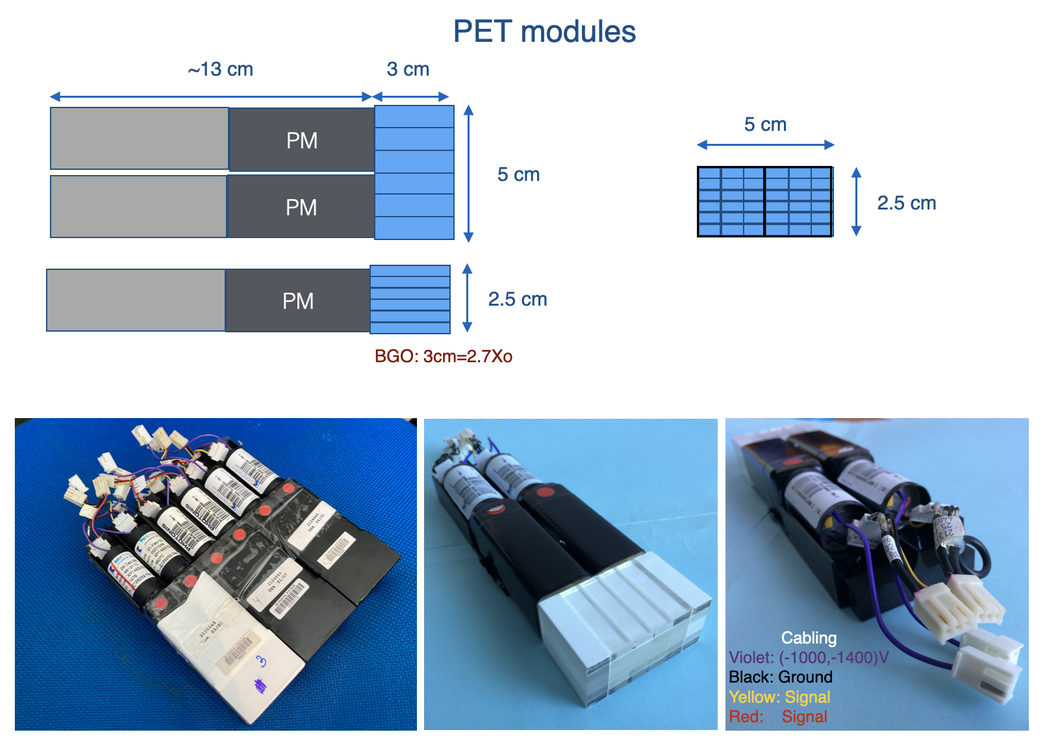
\includegraphics[width=0.75\textwidth]{images/bgo_dimensions.png}'
    \end{figure}
\end{frame}

\begin{columnframe}{Signal characteristics}
    \begin{column}{0.5\textwidth}
        \begin{figure}
            \centering
            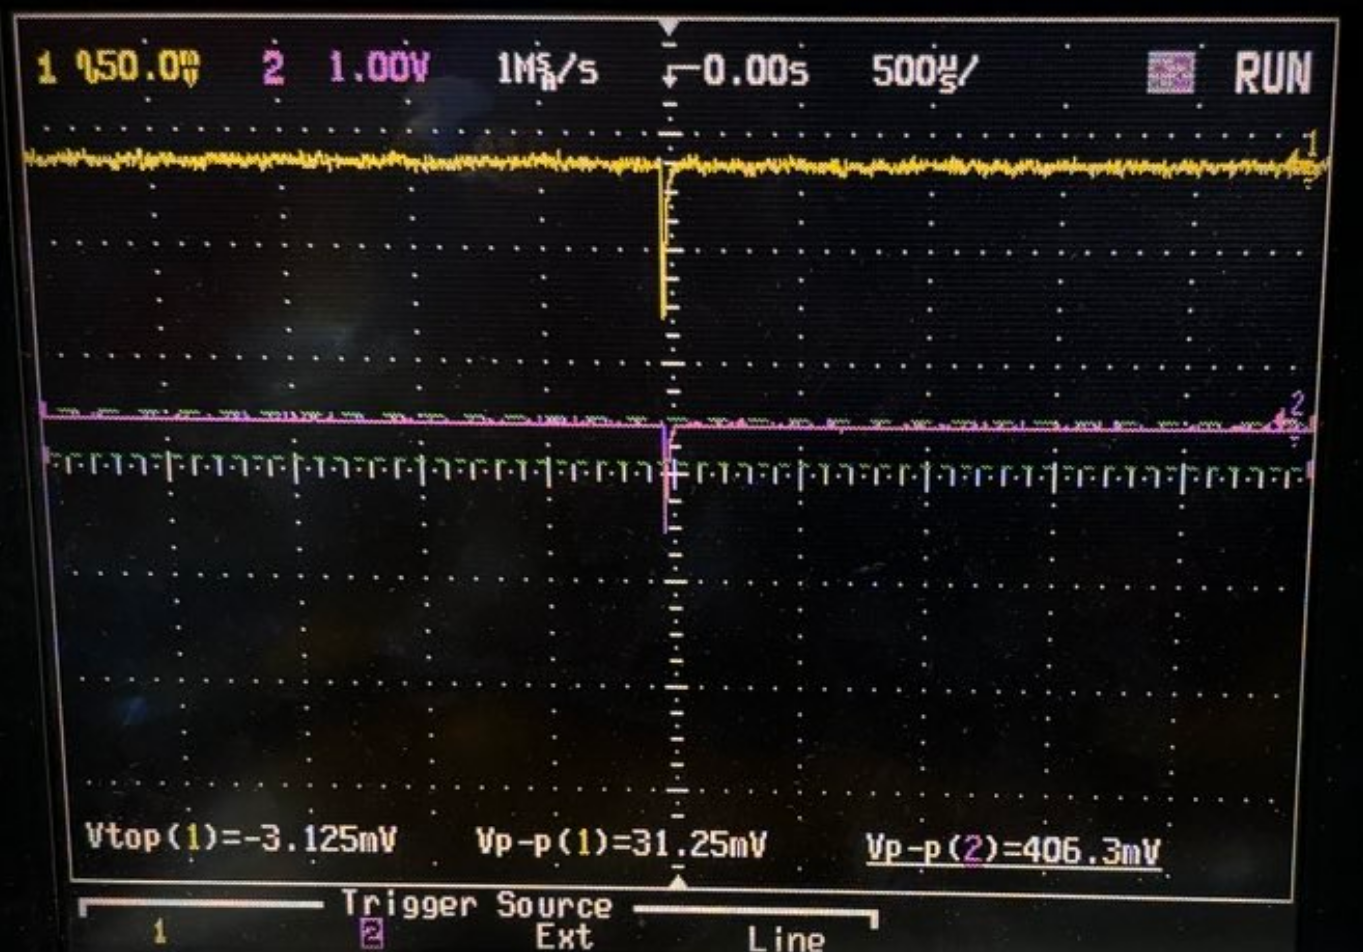
\includegraphics[width=0.9\textwidth]{images/scope_screenshot.png}
        \end{figure}
    \end{column}
    \begin{column}{0.5\textwidth}
        \begin{itemize}
            \item When connected directly to the scope, the signal is about \SI{1}{\volt} in amplitude. It has a length in microseconds.
            \item The constant voltage offset is about \SI{7}{\volt}.
            \item The tube must be supplied with a high voltage of about \SI{1400}{\volt}.
        \end{itemize}
    \end{column}
\end{columnframe}

\begin{frame}{PET machine design considerations note}
    The tubes were designed for a PET machine, which means their signal does not necessarily need to have a high energy resolution. The main goal is to detect the presence of a photon (known to be at 511 \keV from the $e^+ - e^-$ annihilation), not to measure its energy. These detectors were arranged in a ring around the patient, and the signal was used to determine the position of the annihilation event. It is therefore possible that the energy resolution is not good enough for spectroscopy.
\end{frame}

% BGOs
% pmt's - electrical 

\section{Previous work + Issues}
\begin{columnframe}{What has been done}
    \begin{column}{0.5\textwidth}
        \begin{figure}
            \centering
            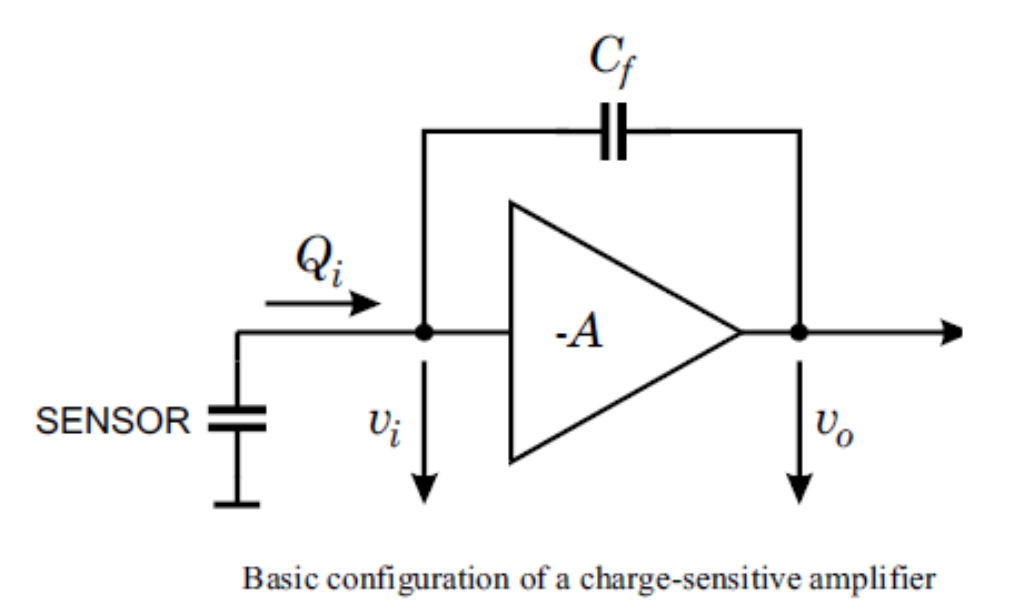
\includegraphics[width=0.9\textwidth]{images/csp_schematic.png}
        \end{figure}
    \end{column}
    \begin{column}{0.5\textwidth}
        \begin{itemize}
            \item we managed to get a signal from the tubes
            \item the signal is high impedance, which means it requires a preamplifier (charge sensitive preamplifier, pictured left)
        \end{itemize}
    \end{column}
\end{columnframe}

\begin{frame}{Measurement setup}
    \begin{figure}
        \centering
        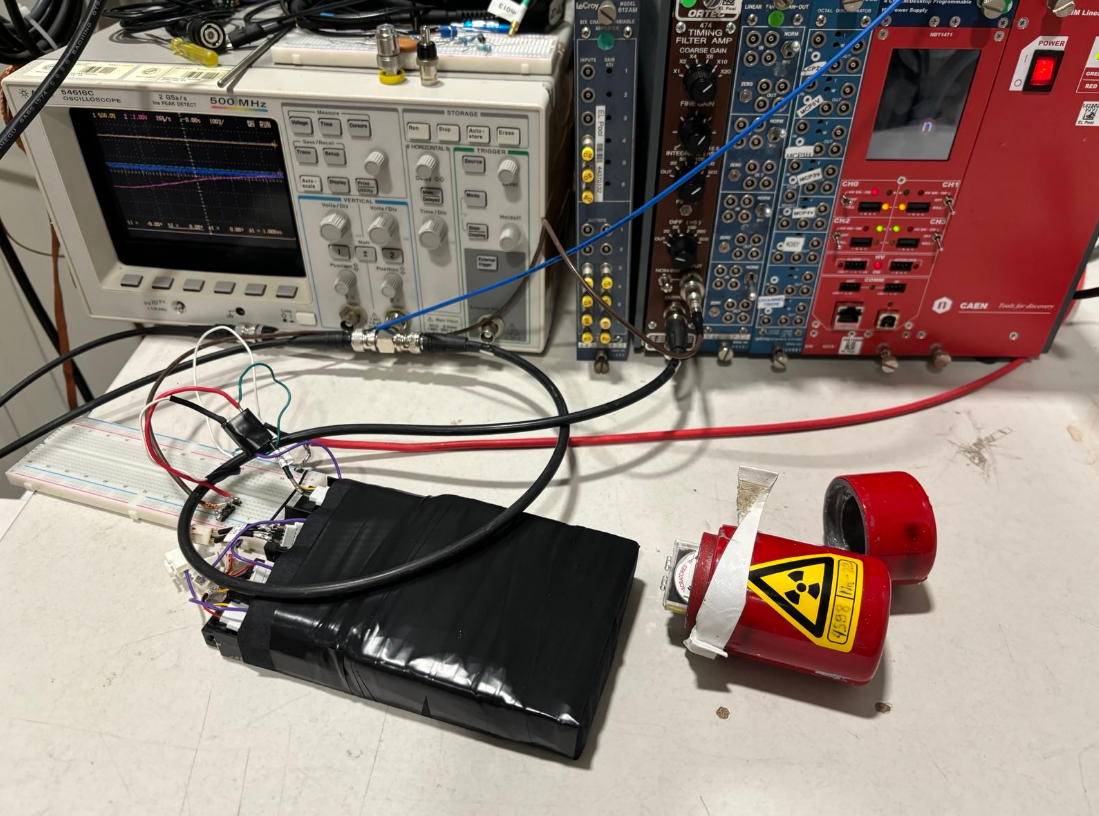
\includegraphics[width=0.8\textwidth]{images/measurement_setup.png}
    \end{figure}

\end{frame}

\begin{columnframe}{Measurement setup}
    \begin{column}{0.5\textwidth}
        \begin{figure}
            \centering
            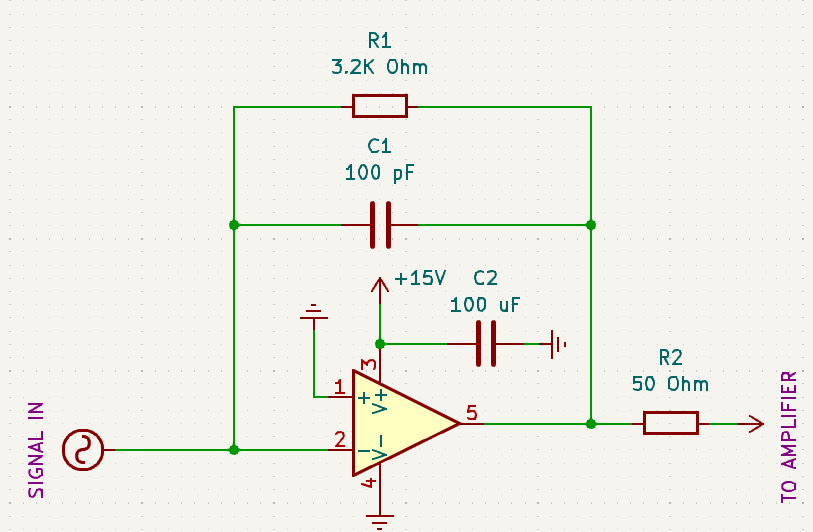
\includegraphics[width=0.9\textwidth]{images/schematic_csp.png}
        \end{figure}
    \end{column}
    \begin{column}{0.5\textwidth}
        \begin{itemize}
            \item preamp: designed by me, based on the schematic from the previous slide, using generic 8082IN op-amp
            \item oscilloscope: 54616C, 500 MHz, 2 GSa/s
            \item power supply: CAEN,  1400 V, 1 mA
            \item DAQ: CAEN DT5720D - 4 Ch. 12 bit 250 MS/s Digitizer: 10MS/ch, C20, SE
        \end{itemize}
    \end{column}
\end{columnframe}

\begin{columnframe}{Available sources}
    \begin{column}{0.5\textwidth}
        \begin{figure}
            \centering
            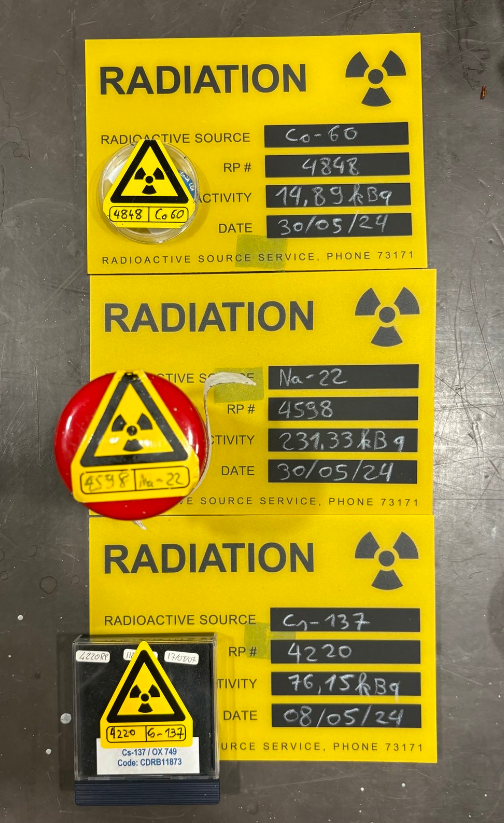
\includegraphics[width=0.7\textwidth]{images/radioactive_sources.png}
        \end{figure}
    \end{column}
    \begin{column}{0.5\textwidth}
        \begin{itemize}
            \item we have access to three radioactive sources: \ce{^{22}Na}, \ce{^{137}Cs}, and \ce{^{60}Co}
        \end{itemize}
    \end{column}
\end{columnframe}

\begin{frame}{Results: background (raw)}
    \begin{figure}
        \centering
        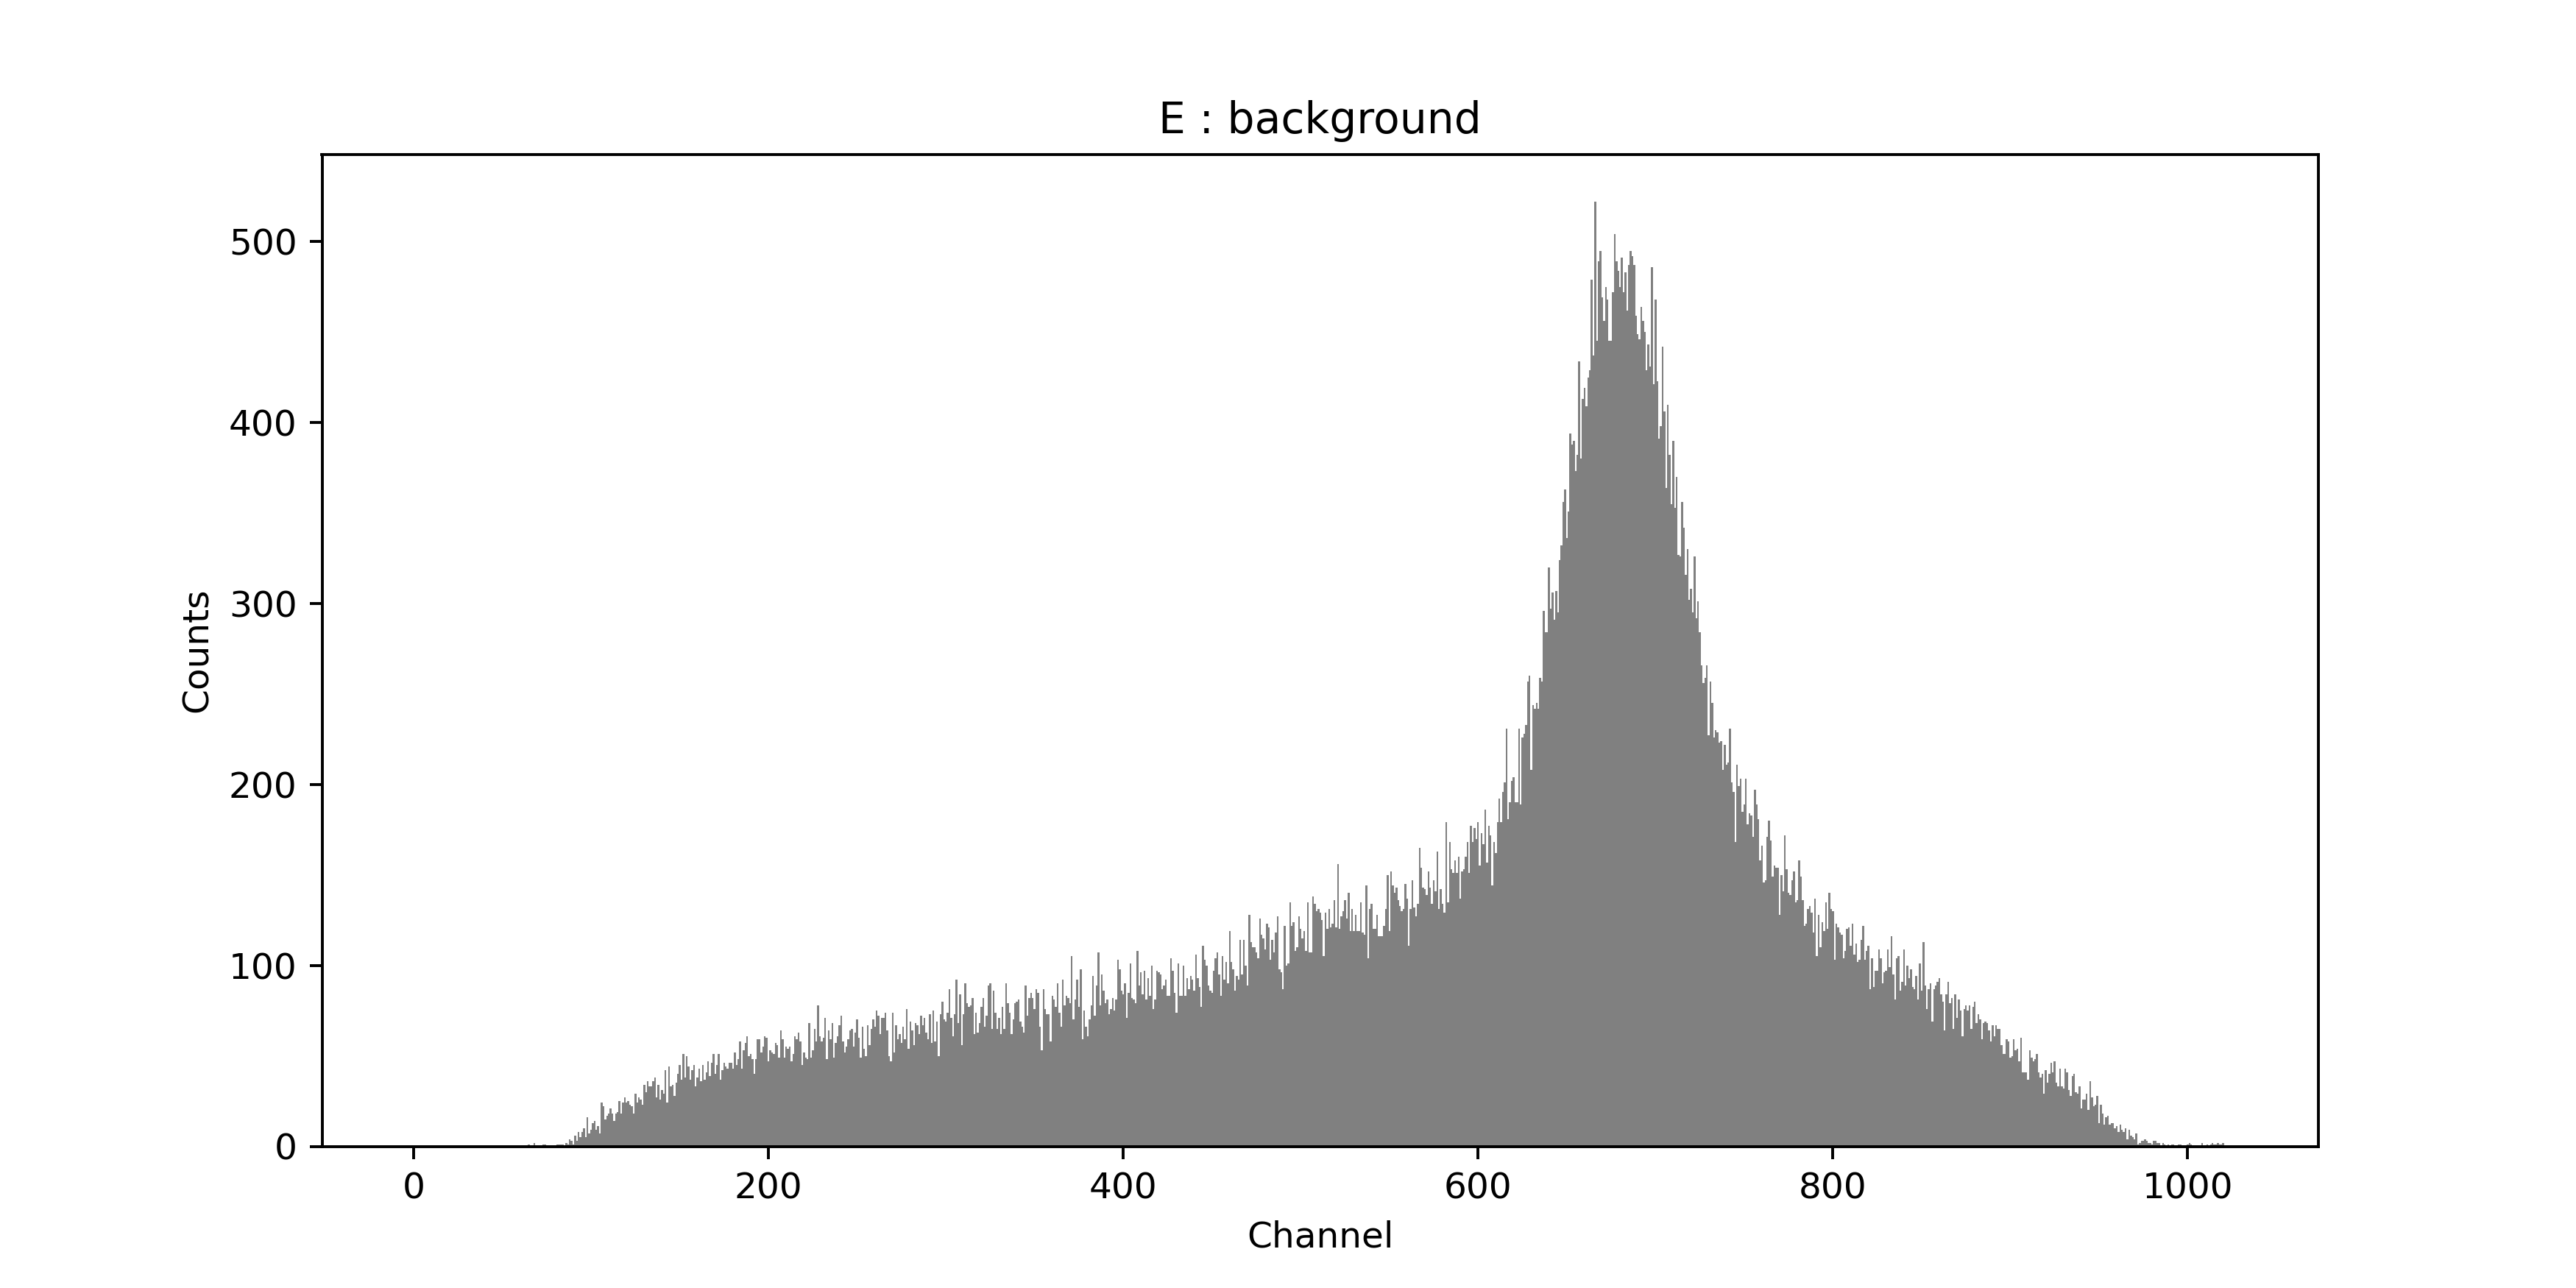
\includegraphics[width=0.7\textwidth]{images/background.png}
    \end{figure}
\end{frame}

\begin{frame}{Results: sources (raw)}
    \begin{figure}
        \centering
        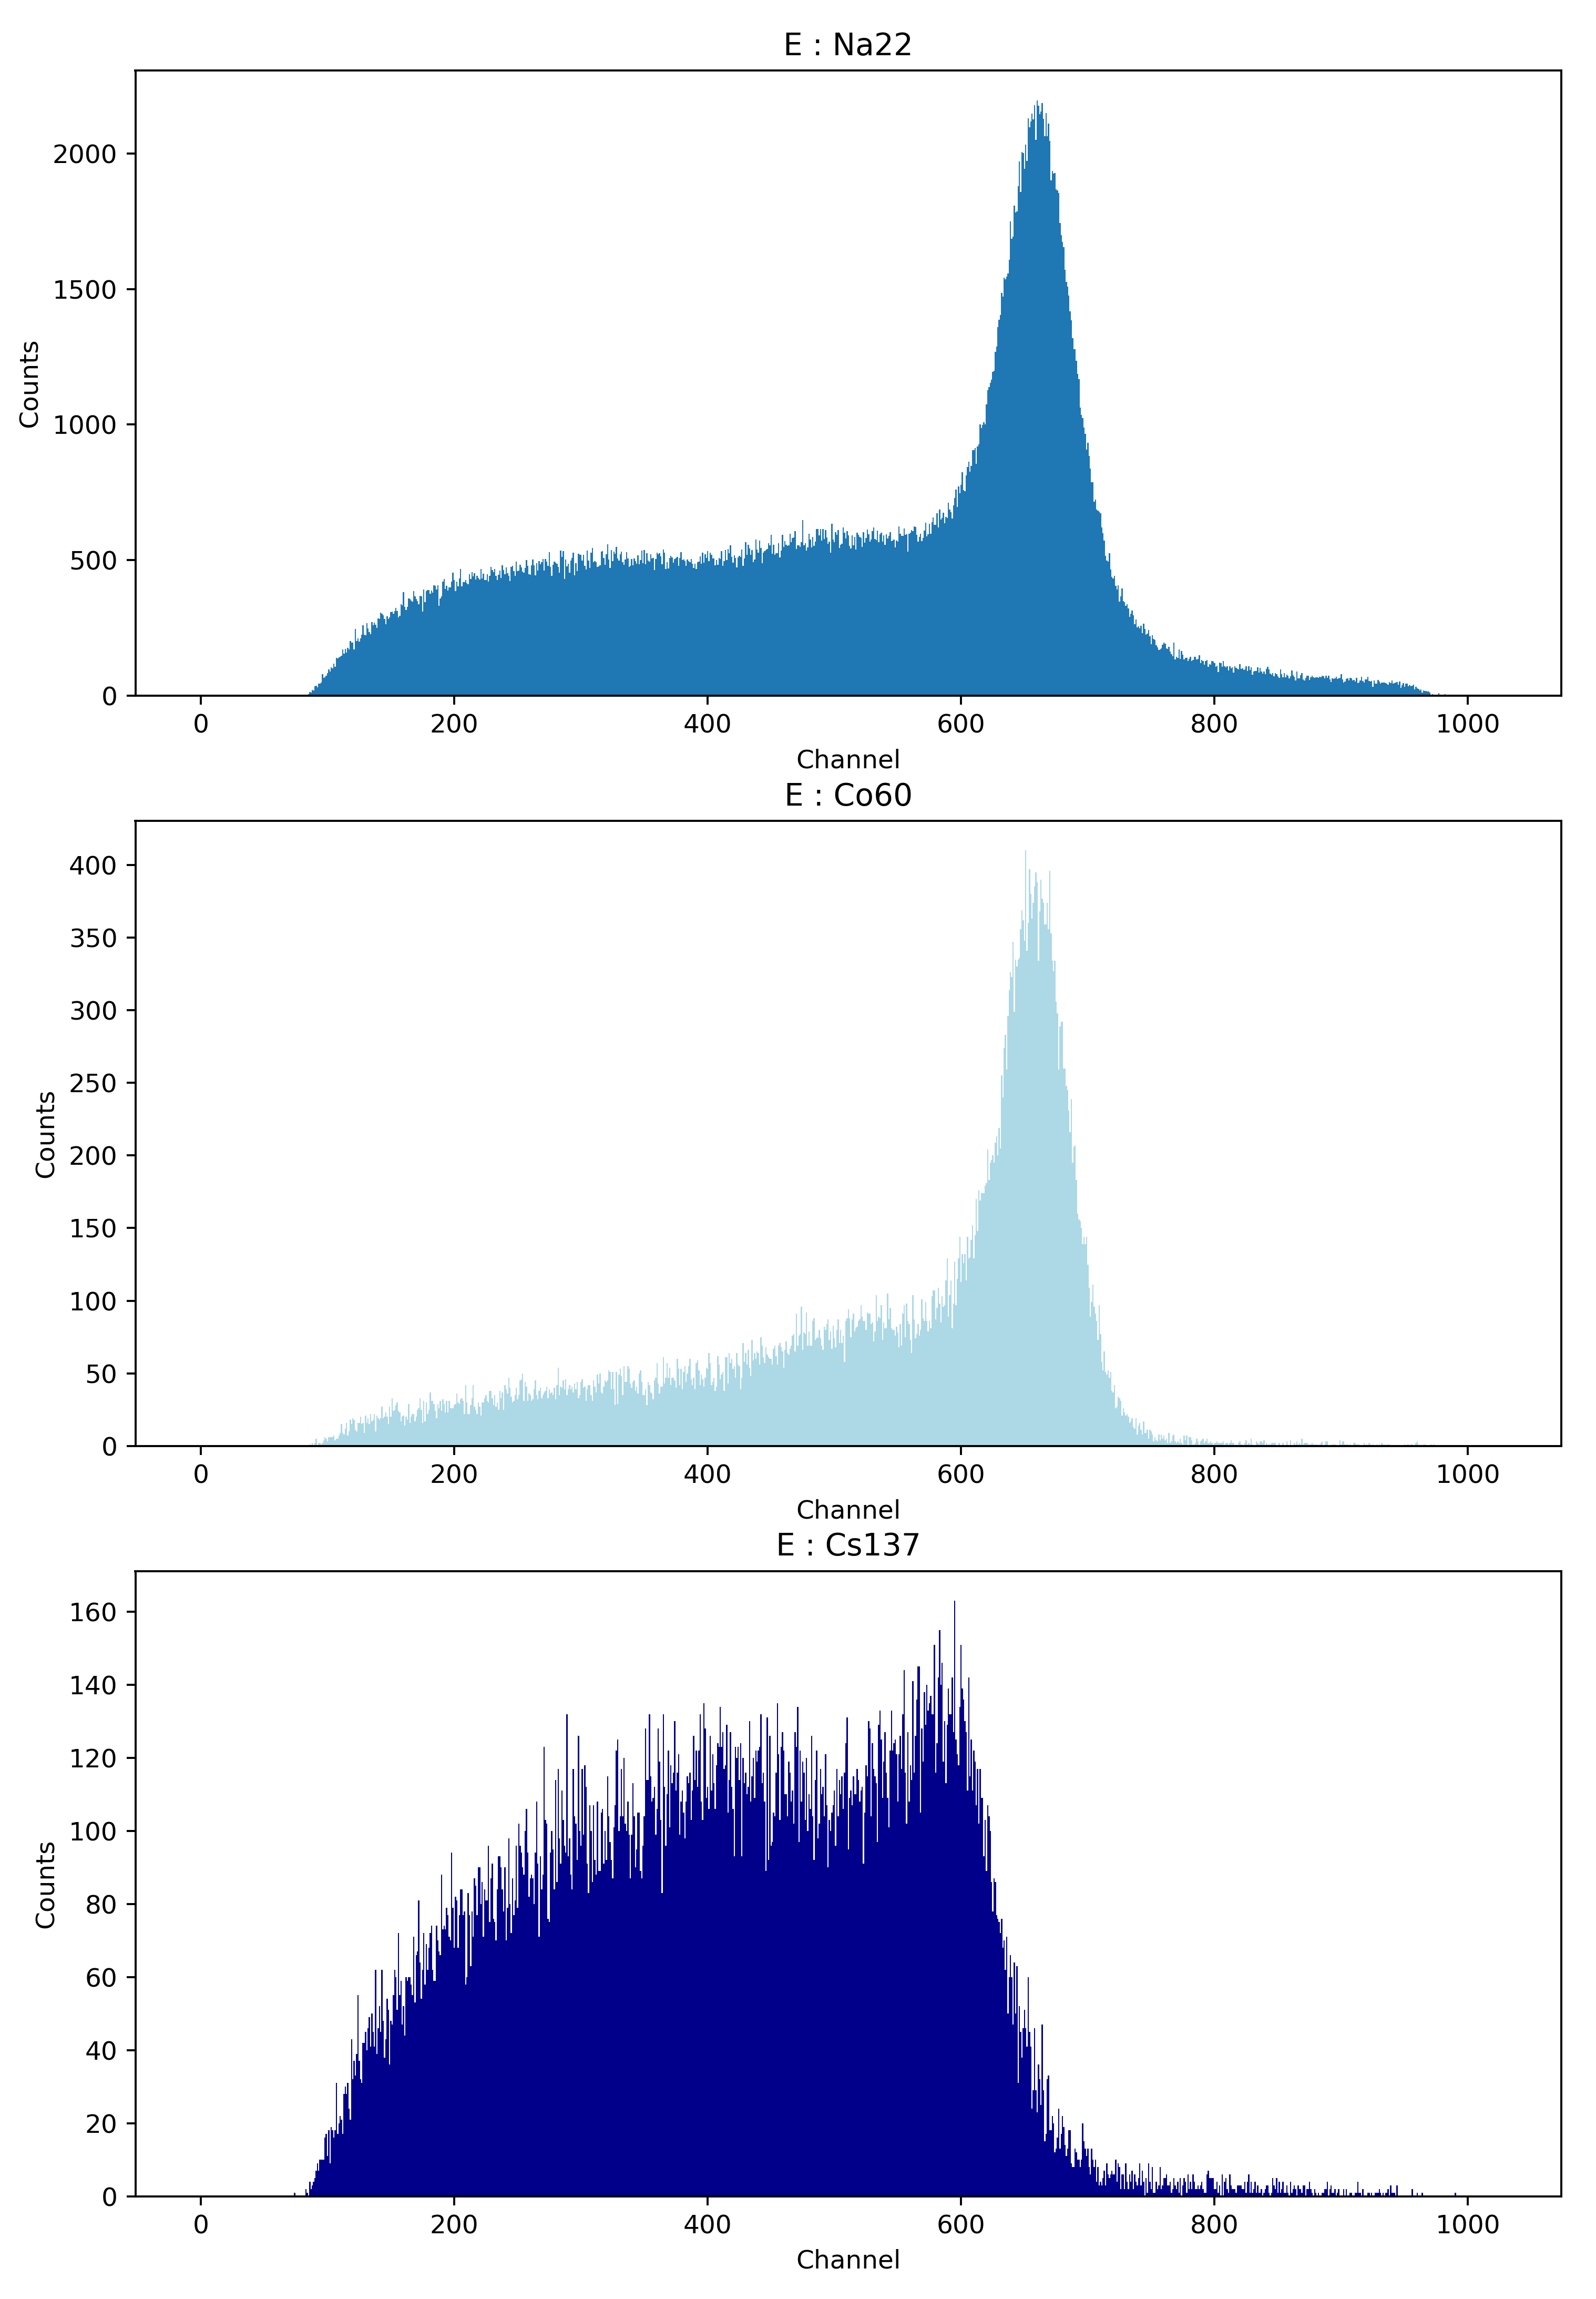
\includegraphics[width=0.45\textwidth]{images/spectra_raw.png}
    \end{figure}
\end{frame}

\begin{frame}{Results: sources (background subtracted, corrected for exposure time, activity)}
    \begin{figure}
        \centering
        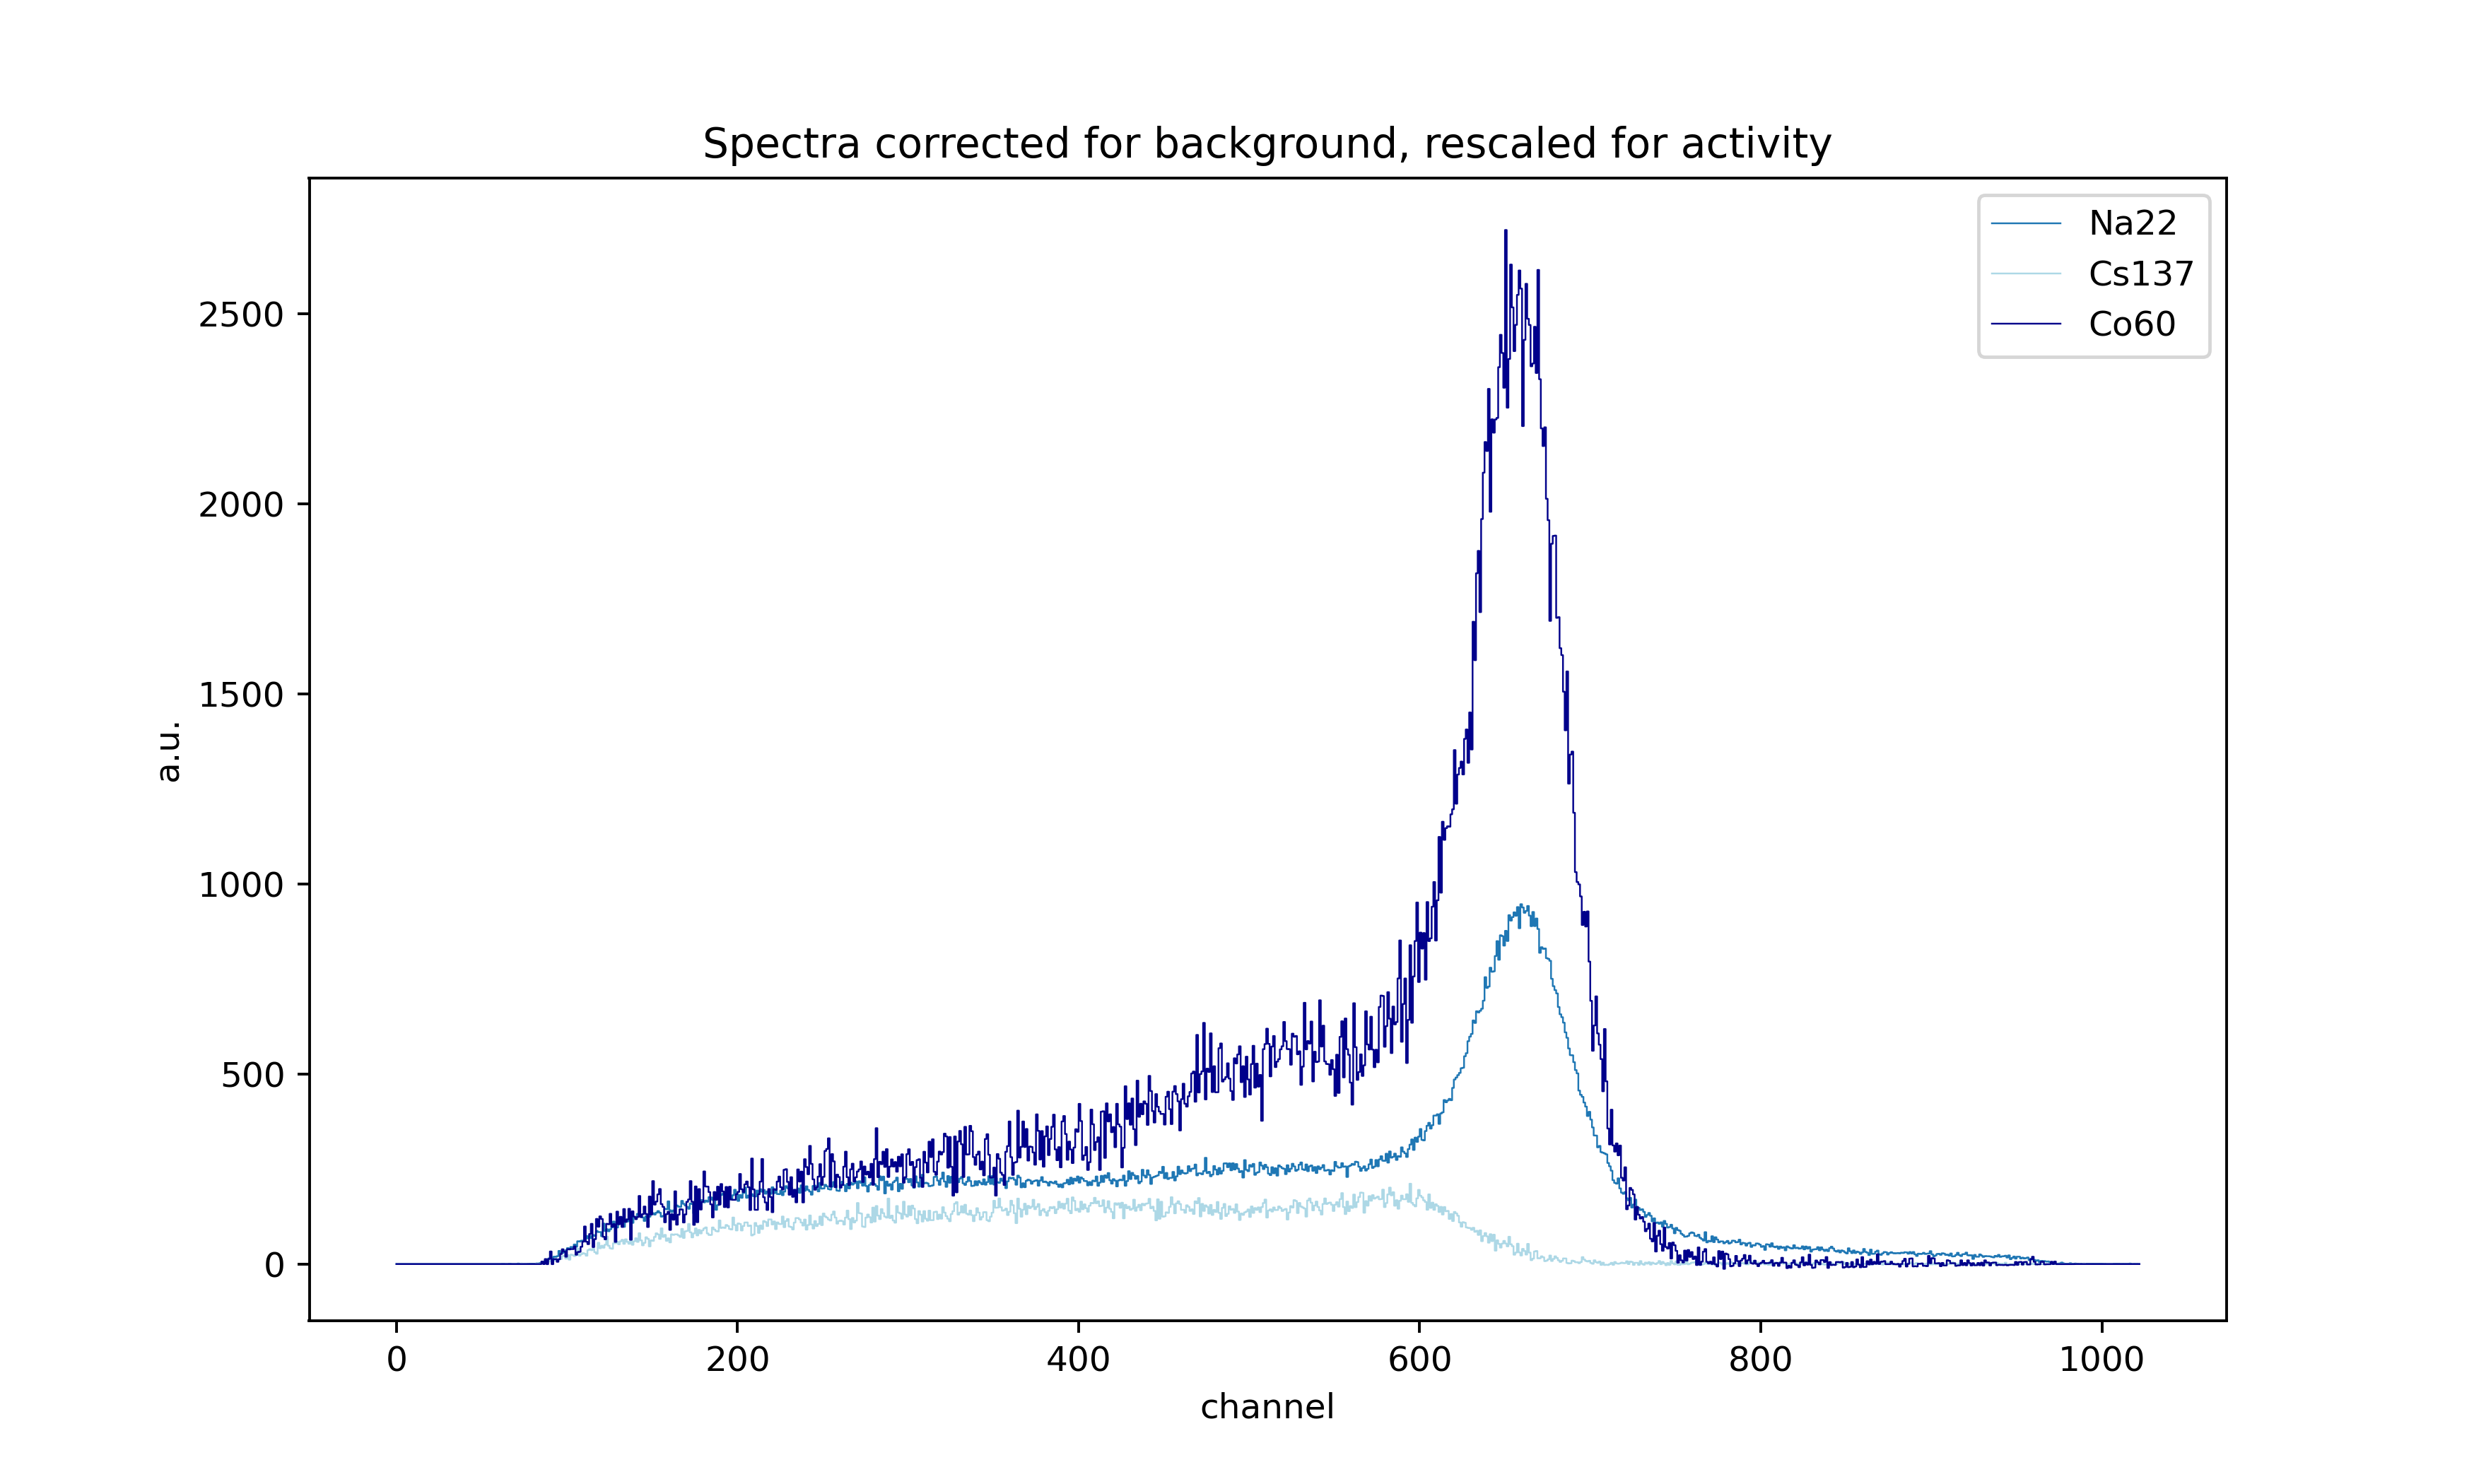
\includegraphics[width=0.7\textwidth]{images/spectra_adjusted.png}
    \end{figure}
\end{frame}

\begin{frame}{Results: Expected Na22 spectrum}
    \begin{figure}
        \centering
        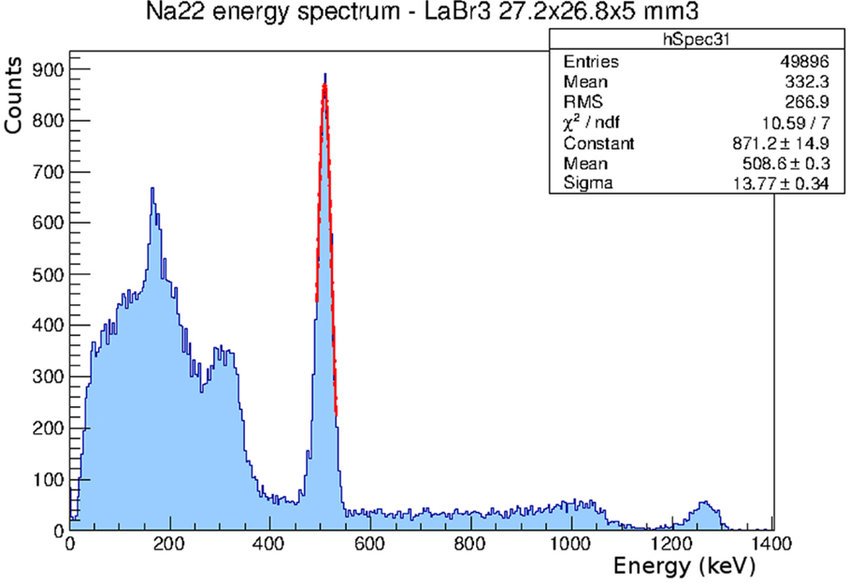
\includegraphics[width=0.7\textwidth]{images/Na22_expected_spectrum.jpg}
    \end{figure}
\end{frame}

\begin{frame}{Results: Expected Cs137 spectrum}
    \begin{figure}
        \centering
        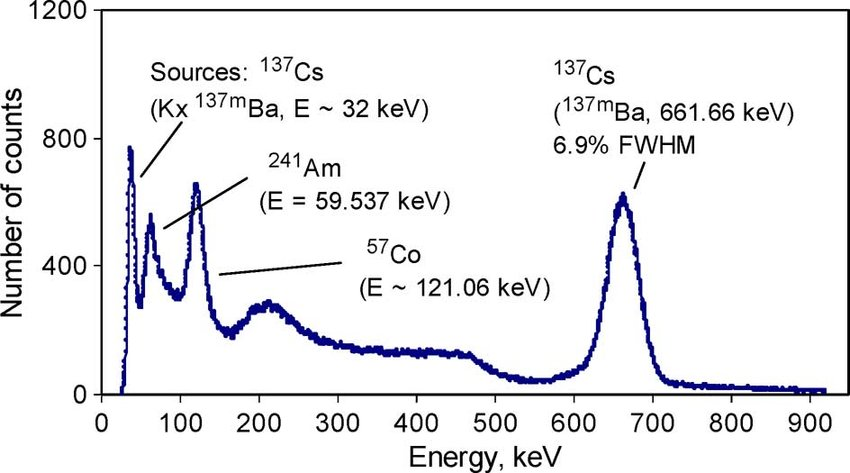
\includegraphics[width=0.7\textwidth]{images/Cs137_expected_spectrum.jpg}
    \end{figure}
\end{frame}

\begin{frame}{Results: Expected Co60 spectrum}
    \begin{figure}
        \centering
        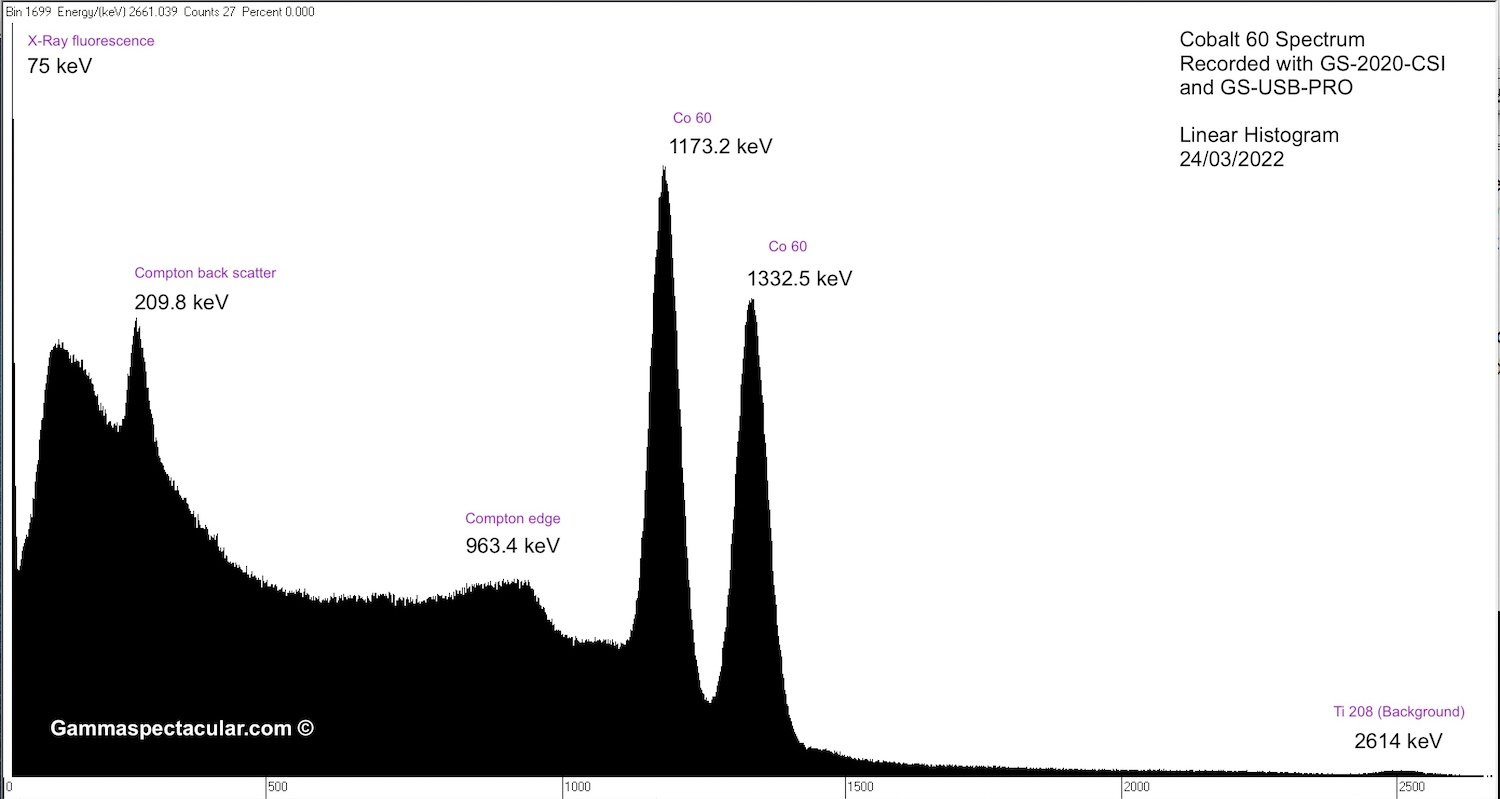
\includegraphics[width=0.9\textwidth]{images/Co60_expected_spectrum.png}
    \end{figure}
\end{frame}

\begin{frame}{Results summary}
    As we can see, the measurement setup behaved differently for each isotope, however exhibits no discernible features/similarities to the expected spectra. This is likely due to the low energy resolution of the detector, but might also be simply due to user (my) error/poor preamp design, or DAQ integration.

    We have no documentation on the tubes, so we do not know their resolution. Moreover we do not know the state of the crystals themselves. This is why I was inclined to attach them to a known detector (SIPM would likely be easiest) and see if we can isolate the issue.
\end{frame}

% Trying to design a preamp
% Results: raw spectra
% Results: corrected spectra

\section{Plans}

\begin{columnframe}{Main plan}
    \begin{column}{0.5\textwidth}
        \begin{figure}
            \centering
            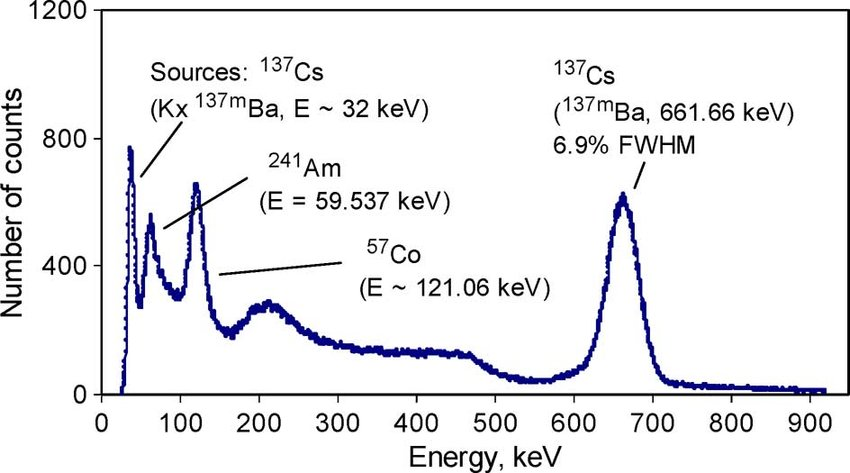
\includegraphics[width=0.95\textwidth]{images/Cs137_expected_spectrum.jpg}
        \end{figure}
    \end{column}
    \begin{column}{0.5\textwidth}
        \begin{itemize}
            \item The main goal is to characterise the PMT detector in terms of energy and time resolution.
            \item If we manage to get discernible spectra from the sources at room temperature, this will already be considered a success. We were planning on calibrating the detector based on the location of the photopeaks in channel-space.
        \end{itemize}
    \end{column}
\end{columnframe}

\begin{columnframe}{Plan B - investigate the crystals}
    \begin{column}{0.5\textwidth}
        \begin{figure}
            \centering
            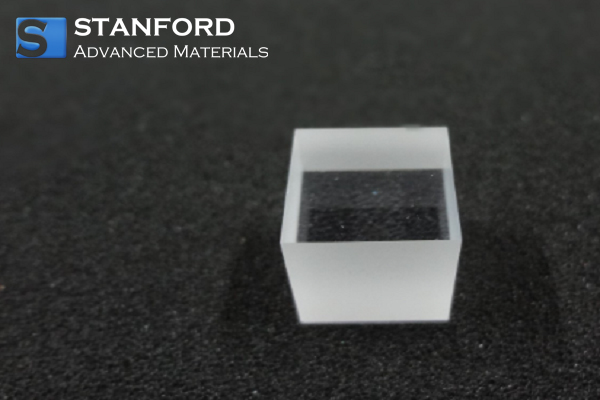
\includegraphics[width=0.7\textwidth]{images/bgo-scintillation-crystal_stanford.jpg}
        \end{figure}
    \end{column}
    \begin{column}{0.5\textwidth}
        \begin{itemize}
            \item If we fail to get the tubes to act as expected, the next step would be to take the crystals out of the tubes and attach them to a known detector.
            \item This approach might also simplify preampifier design, since modern SiPM's should be better-documented.
        \end{itemize}
    \end{column}
\end{columnframe}

\begin{columnframe}{Nice-to-have: Temperature characteristic}
    \begin{column}{0.5\textwidth}
        \begin{figure}
            \centering
            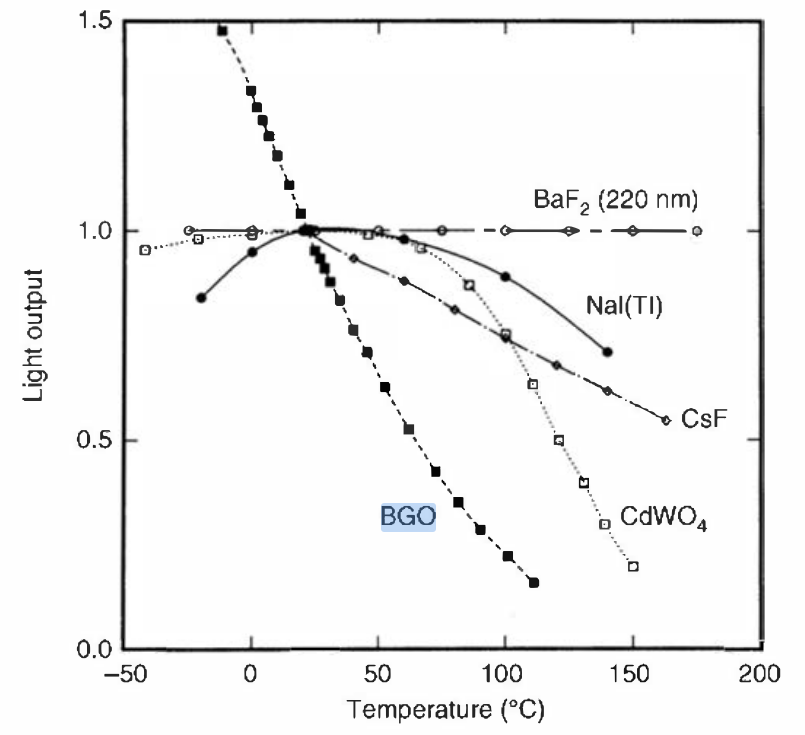
\includegraphics[width=0.7\textwidth]{images/BGO_and_others_light_temp.png}
        \end{figure}
    \end{column}
    \begin{column}{0.5\textwidth}
        If the tubes turn out to work well at room temperature (or if we manage to get them working with another detector), we could try to cool them down to Your capabilities (I think You've mentioned -25 C). We would expect the time resolution to improve and the light yield should increase (but no more than 1.5x fold).
    \end{column}
\end{columnframe}

\begin{frame}{Thoughts on the muon source}
    I have not yet had the opportunity to work with a muon source. However, I would expect the signal peaks to be much larger in this case. We would observe this without a source and attribute it to cosmic radiation. The peaks would reach up to 7 Volts (!). If this is possible to try without risking the equipment (mainly worried about the DAQ), I would be very interested in seeing the results.

\end{frame}



% main plan: find the energy+time range and resolution of the detector 
% side quests: put the working detector setup in the cold and see if it behaves better
% side quests: hook up an SIPM to the crystals themselves

\setbeamertemplate{headline}{}
\setbeamertemplate{footline}{}
\begin{frame}{}
    \centering
    \Large{Thank you for your attention}
\end{frame}


\end{document}